%%%% 補助スライド
\appendix
\backupbegin

\begin{frame}{~}
 \centering
 - 補足用 -
\end{frame} 
%%%%%%%%%%%%%%%%%%%%%%%%%%%%%%%%%%%%%%%%%%%%%%%%%%
%% 配電網問題の例
%%%%%%%%%%%%%%%%%%%%%%%%%%%%%%%%%%%%%%%%%%%%%%%%%%
\begin{frame}{配電網問題の例}
 
 \begin{block}{配電網問題}
  与えられた配電網$D=(S,SW)$から,以下の制約を満たす
  配電網の構成(スイッチの開閉状態$X$)が存在するかどうかを判定する問題.
%  \vspace{-0.5em}
 \begin{itemize}\small
  \item $X ~\textrm{によって定まる配電網構成に停電と短絡が発生しない}$ (\textbf{トポロジ制約})
  \item $J_i = \displaystyle\sum_{j\in S_i^{down}} I_j, \quad J_i \leq J^{max} 
        \quad (\forall s_{i}\in S)\qquad\qquad\qquad\qquad\quad~~$ (\textbf{電流制約})
 \end{itemize}
 \end{block}
  \begin{columns}
    \begin{column}{0.45\textwidth}\centering
      \begin{exampleblock}{入力例}
	\centering
	\scalebox{0.3}{%%%%%%%%%%%%%%%%%%%%%%%%%%%%%%%%%%%%%%%%%%%%%%%%%%
% 配電網 例 (第1章で使う)
%%%%%%%%%%%%%%%%%%%%%%%%%%%%%%%%%%%%%%%%%%%%%%%%%%

\begin{tikzpicture}

 % setting
 \tikzset{customer/.style={rectangle,thick,draw=black,minimum size=0.5cm}}
 \tikzset{on_switch/.style={rectangle,fill=black}}
 \tikzset{off_switch/.style={rectangle,draw=black,fill=white}}
 
 \tikzset{node distance =1cm};

 % substation (x, y, label)
 \newcommand{\substation}[3]{
 \draw [very thick] (#1,#2) circle [radius=0.225cm] node[draw=white,minimum size=1cm](#3){};
 \draw [very thick] (#1+0.225,#2)--(#1+0.35,#2)--(#1+0.35,#2+0.3);
 \draw [very thick] (#1-0.225,#2)--(#1-0.35,#2)--(#1-0.35,#2-0.3);
 \draw [very thick] (#1,#2+0.225)--(#1,#2+0.35);
 \draw [very thick] (#1,#2-0.225)--(#1,#2-0.35);
 \draw [very thick] [domain=-0.284:-0.159] plot(\x+#1,\x+#2);
 \draw [very thick] [domain=0.159:0.284] plot(\x+#1,\x+#2);
 \draw [very thick] [domain=-0.284:-0.159] plot(\x+#1,-\x+#2);
 \draw [very thick] [domain=0.159:0.284] plot(\x+#1,-\x+#2);
 }

 %switch node (position, label, cap)
 %% right switch
 \newcommand{\swnodeR}[4]{
 \coordinate[#1] (#2);
 \node[#1,customer] (#2){#4};
 \node[circle, draw=black, text width=0.2cm, 
 right=0cm of #2, scale=0.3, thick] {};
 \node[right=0cm of #2,scale=0.3, minimum size=0.8cm] (#3){};
 }
 %% left switch
 \newcommand{\swnodeL}[4]{
 %\coordinate[#1] (#2);
 \node[#1,customer] (#2){#4};
 \node[circle, draw=black, fill=white, text width=0.2cm, 
 left=0cm of #2, scale=0.3, thick] (#3){};
 }
 % above switch
 \newcommand{\swnodeA}[4]{
 \coordinate[#1] (#2);
 \node[#1,customer] (#2){#4};
 \node[circle, draw=black, text width=0.2cm, 
 above=0cm of #2, scale=0.3, thick] (#3){};
 }
 % below switch
 \newcommand{\swnodeB}[4]{
 \coordinate[#1] (#2);
 \node[#1,customer] (#2){#4};
 \node[circle, draw=black, text width=0.2cm, 
 below=0cm of #2, scale=0.3, thick] {};
 \node[below=0cm of #2,scale=0.3,minimum size=0.8cm] (#3){};
 }
 
 \substation{0}{0}{sub};
 
 % root1
 \node[customer,fill=black!40,below =4.5cm of sub] (root1) { };
 \swnodeL{left =of root1}{node1}{sw1}{ };
 
 \swnodeR{left=of node1}{node2}{sw2}{ };
 \node[customer,left=of node2] (junc1){ };
 \swnodeL{left =of junc1}{node3}{sw3}{ };
 \swnodeA{above= of junc1}{node4}{sw4}{ }

 \swnodeR{left=of node3}{node5}{sw5}{ };
 \swnodeA{above =of node5}{node6}{sw6}{ };

 \swnodeB{above =of node6}{node7}{sw7}{ };
 \swnodeA{above =of node7}{node29}{sw29}{ };

 \swnodeB{above =of node29}{node30}{sw30}{ };
 
 \swnodeB{above =of node4}{node8}{sw8}{ };
 \swnodeA{above =of node8}{node31}{sw31}{ };
 
 \swnodeB{above =of node31}{node32}{sw32}{ };

 \swnodeR{right =of root1}{node17}{sw17}{ };

 \swnodeL{right =of node17}{node18}{sw18}{ };

 % root2
 \node[customer,fill=black!10,above=4.5cm of sub] (root2) { };
 \swnodeL{left =of root2}{node9}{sw9}{ };

 \swnodeR{left=of node9}{node10}{sw10}{ };
 \node[customer,left=of node10] (junc2){ };
 \swnodeL{left =of junc2}{node11}{sw11}{ };
 \swnodeB{below =of junc2}{node12}{sw12}{ };
 
 \swnodeR{left =of node11}{node13}{sw13}{ };
 \swnodeB{below =of node13}{node14}{sw14}{ };
 
 \swnodeA{below =of node14}{node15}{sw15}{ };

 \swnodeA{below =of node12}{node16}{sw16}{ };

 \swnodeR{right =of root2}{node22}{sw22}{ };

 \swnodeL{right =of node22}{node23}{sw23}{ };
 
 % root3
 \node[customer,pattern=north east lines,right=5.2cm of sub] (root3) { };
 \swnodeB{below =1.4of root3}{node24}{sw24}{ };
 \swnodeA{above =1.4of root3}{node25}{sw25}{ };

 \swnodeA{below =of node24}{node19}{sw19}{ };
 \swnodeL{below =1.3of node19}{node20}{sw20}{ };
 
 \swnodeR{left =of node20}{node21}{sw21}{ };

 \swnodeB{above =of node25}{node26}{sw26}{ };
 \swnodeL{above =1.3of node26}{node27}{sw27}{ };

 \swnodeR{left =of node27}{node28}{sw28}{ };
 
 % sections
 \foreach \v / \u / \t in {root1/sub/$s_a$,root1/node1/$s_1$,node2/junc1/$s_2$, %
 junc1/node3/$s_3$,junc1/node4/$s_4$,node5/node6/$s_5$,node7/node29/$s_6$,node30/node15/$s_7$, %
 sub/root2/$s_b$,root2/node9/$s_8$,node10/junc2/$s_9$,junc2/node11/$s_{10}$,node12/junc2/$s_{11}$, %
 node14/node13/$s_{12}$,node8/node31/$s_{13}$,node32/node16/$s_{14}$,node17/root1/$s_{15}$, %
 node22/root2/$s_{16}$,root3/sub/$s_c$,node24/root3/$s_{17}$,root3/node25/$s_{18}$, %
 node20/node19/$s_{19}$,node26/node27/$s_{20}$,node21/node18/$s_{21}$,node28/node23/$s_{22}$} %
 \draw[thick] (\v) --  node[auto=right]{\t} (\u);

 % switches
 %% horizontal
 \foreach \v / \u / \t in {sw1/sw2/$sw_{1}$,sw3/sw5/$sw_{2}$,sw9/sw10/$sw_{11}$,sw11/sw13/$sw_{12}$,sw18/sw17/$sw_{13}$,
 sw23/sw22/$sw_{15}$,sw20/sw21/$sw_{14}$,sw27/sw28/$sw_{16}$}
 \draw[very thick] (\v) -- node[below=0.2of \v]{\t} (\u.45);
 %% vertical
 \foreach \v / \u / \t in {sw4/sw8/$sw_{4}$,sw6/sw7/$sw_{3}$,sw29/sw30/$sw_{5}$,sw31/sw32/$sw_{6}$,sw15/sw14/$sw_{7}$,%
 sw16/sw12/$sw_{8}$,sw19/sw24/$sw_{9}$,sw25/sw26/$sw_{10}$}
 \draw[very thick] (\v) -- node[auto=below]{\t~~~~~~~~~~} (\u.-30);

\end{tikzpicture}

%%%%%%%%%%%%%%%%%%%%%%%%%%%%%%%%%%%%%%%%%%%%%%%%%%%%%%%%%%
%%% Local Variables:
%%% mode: japanese-latex
%%% TeX-master: paper.tex
%%% End:
}
      \end{exampleblock}
    \end{column}
    \begin{column}{0.05\textwidth}\centering
      $\Rightarrow$
    \end{column}
    \begin{column}{0.45\textwidth}\centering
      \begin{exampleblock}{解の例}
        \centering
        \scalebox{0.3}{\input{tikz/tikz-test-output}}
      \end{exampleblock}
    \end{column}
  \end{columns}
\end{frame}
%%%%%%%%%%%%%%%%%%%%%%%%%%%%%%%%%%%%%%%%%%%%%%%%%%
%% 配電網遷移問題の例
%%%%%%%%%%%%%%%%%%%%%%%%%%%%%%%%%%%%%%%%%%%%%%%%%%
\begin{frame}{配電網遷移問題の例(1/4)}
 \vfill
 \begin{figure}[t]
  \centering
  \scalebox{0.65}{\input{tikz/tikz-test-core-0}}
  \vspace{-0.1cm}
  \caption*{\structure{$\mathbf{t=0}$ \textbf{(スタート状態)}}}
 \end{figure}
\end{frame}
%
\begin{frame}{配電網遷移問題の例(2/4)}
  \vfill
 \begin{figure}[t]
  \centering
  \scalebox{0.65}{\input{tikz/tikz-test-core-1}}
  \vspace{-0.1cm}
  \caption*{\structure{$\mathbf{t=1}$}}
 \end{figure}
\end{frame}
%
\begin{frame}{配電網遷移問題の例(3/4)}
  \vfill
 \begin{figure}[t]
  \centering\hspace{-0.1cm}
  \scalebox{0.65}{\begin{tikzpicture}

 % setting
 \tikzset{customer/.style={rectangle,thick,draw=black,minimum size=0.5cm}}
 \tikzset{on_switch/.style={rectangle,fill=black}}
 \tikzset{off_switch/.style={rectangle,draw=black,fill=white}}
 
 \tikzset{node distance =1cm};

 % substation (x, y, label)
 \newcommand{\substation}[3]{
 \draw [very thick] (#1,#2) circle [radius=0.225cm] node[draw=white,minimum size=1cm](#3){};
 \draw [very thick] (#1+0.225,#2)--(#1+0.35,#2)--(#1+0.35,#2+0.3);
 \draw [very thick] (#1-0.225,#2)--(#1-0.35,#2)--(#1-0.35,#2-0.3);
 \draw [very thick] (#1,#2+0.225)--(#1,#2+0.35);
 \draw [very thick] (#1,#2-0.225)--(#1,#2-0.35);
 \draw [very thick] [domain=-0.284:-0.159] plot(\x+#1,\x+#2);
 \draw [very thick] [domain=0.159:0.284] plot(\x+#1,\x+#2);
 \draw [very thick] [domain=-0.284:-0.159] plot(\x+#1,-\x+#2);
 \draw [very thick] [domain=0.159:0.284] plot(\x+#1,-\x+#2);
 }

 %switch node (position, label, cap)
 %% right switch
 \newcommand{\swnodeR}[4]{
 \coordinate[#1] (#2);
 \node[#1,customer] (#2){#4};
 \node[circle, draw=black, text width=0.2cm, 
 right=0cm of #2, scale=0.3, thick] {};
 \node[right=0cm of #2,scale=0.3, minimum size=0.8cm] (#3){};
 }
 %% left switch
 \newcommand{\swnodeL}[4]{
 %\coordinate[#1] (#2);
 \node[#1,customer] (#2){#4};
 \node[circle, draw=black, fill=white, text width=0.2cm, 
 left=0cm of #2, scale=0.3, thick] (#3){};
 }
 % above switch
 \newcommand{\swnodeA}[4]{
 \coordinate[#1] (#2);
 \node[#1,customer] (#2){#4};
 \node[circle, draw=black, text width=0.2cm, 
 above=0cm of #2, scale=0.3, thick] (#3){};
 }
 % below switch
 \newcommand{\swnodeB}[4]{
 \coordinate[#1] (#2);
 \node[#1,customer] (#2){#4};
 \node[circle, draw=black, text width=0.2cm, 
 below=0cm of #2, scale=0.3, thick] {};
 \node[below=0cm of #2,scale=0.3,minimum size=0.8cm] (#3){};
 }
 
 \substation{0}{0}{sub};
 
 % root1
 \node[customer,fill=black!40,below =4.5cm of sub] (root1) { };
 \swnodeL{left =of root1,fill=black!40}{node1}{sw1}{ };
 
 \swnodeR{left=of node1,fill=black!40}{node2}{sw2}{ };
 \node[customer,left=of node2,fill=black!40] (junc1){ };
 \swnodeL{left =of junc1,fill=black!40}{node3}{sw3}{ };
 \swnodeA{above= of junc1,fill=black!40}{node4}{sw4}{ }

 \swnodeR{left=of node3,fill=black!40}{node5}{sw5}{ };
 \swnodeA{above =of node5,fill=black!40}{node6}{sw6}{ };

 \swnodeB{above =of node6,fill=black!40}{node7}{sw7}{ };
 \swnodeA{above =of node7,fill=black!40}{node29}{sw29}{ };

 \swnodeB{above =of node29,fill=black!10}{node30}{sw30}{ };
 
 \swnodeB{above =of node4,fill=black!40}{node8}{sw8}{ };
 \swnodeA{above =of node8,fill=black!40}{node31}{sw31}{ };
 
 \swnodeB{above =of node31,fill=black!10}{node32}{sw32}{ };

 \swnodeR{right =of root1,fill=black!40}{node17}{sw17}{ };

 \swnodeL{right =of node17,fill=black!40}{node18}{sw18}{ };

 % root2
 \node[customer,fill=black!20,above=4.5cm of sub, fill=black!10] (root2) { };
 \swnodeL{left =of root2,fill=black!10}{node9}{sw9}{ };

 \swnodeR{left=of node9,fill=black!10}{node10}{sw10}{ };
 \node[customer,left=of node10,fill=black!10] (junc2){ };
 \swnodeL{left =of junc2,fill=black!10}{node11}{sw11}{ };
 \swnodeB{below =of junc2,fill=black!10}{node12}{sw12}{ };
 
 \swnodeR{left =of node11,fill=black!10}{node13}{sw13}{ };
 \swnodeB{below =of node13,fill=black!10}{node14}{sw14}{ };
 
 \swnodeA{below =of node14,fill=black!10}{node15}{sw15}{ };

 \swnodeA{below =of node12,fill=black!10}{node16}{sw16}{ };

 \swnodeR{right =of root2,fill=black!10}{node22}{sw22}{ };

 \swnodeL{right =of node22,fill=black!10}{node23}{sw23}{ };
 
 % root3
 \node[customer,fill=black!20,right=5.2cm of sub,pattern=north east lines] (root3) { };
 \swnodeB{below =1.4of root3,pattern=north east lines}{node24}{sw24}{ };
 \swnodeA{above =1.4of root3,pattern=north east lines}{node25}{sw25}{ };

 \swnodeA{below =of node24,pattern=north east lines}{node19}{sw19}{ };
 \swnodeL{below =1.3of node19,pattern=north east lines}{node20}{sw20}{ };
 
 \swnodeR{left =of node20,fill=black!40}{node21}{sw21}{ };

 \swnodeB{above =of node25,fill=black!10}{node26}{sw26}{ };
 \swnodeL{above =1.3of node26,fill=black!10}{node27}{sw27}{ };

 \swnodeR{left =of node27,fill=black!10}{node28}{sw28}{ };
 
 % sections
 \foreach \v / \u / \t in {root1/sub/$s_a$,root1/node1/$s_1$,node2/junc1/$s_2$, %
 junc1/node3/$s_3$,junc1/node4/$s_4$,node5/node6/$s_5$,node7/node29/$s_6$,node30/node15/$s_7$, %
 sub/root2/$s_b$,root2/node9/$s_8$,node10/junc2/$s_9$,junc2/node11/$s_{10}$,node12/junc2/$s_{11}$, %
 node14/node13/$s_{12}$,node8/node31/$s_{13}$,node32/node16/$s_{14}$,node17/root1/$s_{15}$, %
 node22/root2/$s_{16}$,root3/sub/$s_c$,node24/root3/$s_{17}$,root3/node25/$s_{18}$, %
 node20/node19/$s_{19}$,node26/node27/$s_{20}$,node21/node18/$s_{21}$,node28/node23/$s_{22}$} %
 \draw[thick] (\v) --  node[auto=right]{\t} (\u);

 % switches
 %% horizontal
 \foreach \v / \u / \t in {sw1/sw2/$sw_{1}$,sw3/sw5/$sw_{2}$,sw9/sw10/$sw_{11}$,
 sw11/sw13/$sw_{12}$,sw18/sw17/$sw_{13}$,sw23/sw22/$sw_{15}$,sw27/sw28/$sw_{16}$}
 \draw[very thick] (\v) -- node[below=0.2of \v]{\t} (\u.center);
 
 \foreach \v / \u in {sw20/sw21}
 \draw[very thick] (\v) -- (\u.45);
 %% vertical
 \foreach \v / \u / \t in {sw4/sw8/$sw_{4}$,sw6/sw7/$sw_{3}$,sw15/sw14/$sw_{7}$,%
 sw16/sw12/$sw_{8}$,sw19/sw24/$sw_{9}$}
 \draw[very thick] (\v) -- node[auto=below]{\t~~~~~~~~~~} (\u.center);

 \foreach \v / \u in {sw29/sw30,sw31/sw32,sw25/sw26}
 \draw[very thick] (\v) -- (\u.-30);
\end{tikzpicture}

%%%%%%%%%%%%%%%%%%%%%%%%%%%%%%%%%%%%%%%%%%%%%%%%%%%%%%%%%%
%%% Local Variables:
%%% mode: japanese-latex
%%% TeX-master: paper.tex
%%% End:
}
  \vspace{-0.1cm}
  \caption*{\structure{$\mathbf{t=2}$}}
 \end{figure}
\end{frame}
%
\begin{frame}{配電網遷移問題の例(4/4)}
  \vfill
 \begin{figure}[t]
  \centering\hspace{-0.1cm}
  \scalebox{0.65}{\input{tikz/tikz-test-core-3}}
  \vspace{-0.1cm}
  \caption*{\structure{$\mathbf{t=3}$ \textbf{(ゴール状態)}}}
 \end{figure}
\end{frame}

%%%%%%%%%%%%%%%%%%%%%%%%%%%%%%%%%%%%%%%%%%%%%%%%%%
%% 卒業研究
%%%%%%%%%%%%%%%%%%%%%%%%%%%%%%%%%%%%%%%%%%%%%%%%%%
\begin{frame}{配電網問題のASP符号化(卒業研究)}
   %\scalebox{0.9}{\centering\begin{figure*}[t]
  \centering
  \thicklines
  \setlength{\unitlength}{1.28pt}
  \small
  \begin{picture}(280,57)(4,-10)
    \put( -35, 20){\dashbox(70,24){\shortstack{組合せ最適化問題\\のインスタンス}}}
    \put( 45, 20){\framebox(50,24){変換器}}
    \put(105, 20){\dashbox(70,24){\shortstack{ASPファクト}}}
    \put(105,-10){\dashbox(70,24){\shortstack{ASP符号化\\(論理プログラム)}}}
    \put(185,-10){\framebox(60,54){}}
    \put(189, 25){\framebox(52,12){ASPソルバー}}
    \put(190, -5){\framebox(50,12){LNPS}}
    % \put(180, 20){\framebox(50,24){ASPシステム}}
    \put(255, 20){\dashbox(70,24){\shortstack{組合せ最適化問題\\の最適解}}}
    \put(  35, 32){\vector(1,0){10}}
    \put(  95, 32){\vector(1,0){10}}
    \put(175, 32){\vector(1,0){10}}
    \put(245, 32){\vector(1,0){10}}
    \put(175, +2){\line(1,0){4}}
    \put(179, +2){\line(0,1){30}}
    \put(205,  7){\vector(0,1){17}}
    \put(225, 24){\vector(0,-1){17}}
    \put(190, 48){提案ソルバー}
  \end{picture}  
\caption{提案ソルバー\textit{asprior}の構成}
\label{fig:arch}
\end{figure*}

%%% Local Variables: 
%%% mode: latex
%%% TeX-master: "paper"
%%% End: 
}
   \begin{block}{根付き全域森問題の2種類のASP符号化を考案}
     \begin{itemize}
     \item \alert{\bf 基本符号化}
       \begin{itemize}
       \item 根付き全域森問題の制約を,\textbf{ASPのルール7個}で簡潔に記述
       \end{itemize}
     \item \alert{\bf 改良符号化}
       \begin{itemize}
       \item ASPシステムは,変数を含む論理プログラムを,変数を含まない
         論理プログラムに\textbf{基礎化}したのち解集合を計算する.
       \item 根付き連結制約をASPの個数制約で表現することにより,
         \textbf{基礎化後のルール数を少なく抑える}よう工夫されている.
       \item これにより,改良符号化は大規模な問題への有効性が期待できる.
       \end{itemize}
     \end{itemize}
   \end{block}
 \begin{itemize}
  \renewcommand{\thefootnote}{\fnsymbol{footnote}}
  \setcounter{footnote}{1}
  \item \textit{DNET}\footnote{https://github.com/takemaru/dnet},
        および,\textit{Graph Coloring and its Generalizations}
        \footnote{https://mat.tepper.cmu.edu/COLOR04/}%
        の問題をベースに独自に生成した配電網問題を用いて評価実験を行った.
  \item 結果として,改良符号化は,基本符号化と比較して,より多くの問題を高速に解いた.
 \end{itemize}
\end{frame}

%%%%%%%%%%%%%%%%%%%%%%%%%%%%%%%%%%%%%%%%%%%%%%%%%% 
%% 根付き全域森問題
%%%%%%%%%%%%%%%%%%%%%%%%%%%%%%%%%%%%%%%%%%%%%%%%%%
\begin{frame}{根付き全域森問題}
 \begin{alertblock}{}
  トポロジ制約を満たす配電網構成は,グラフと根と呼ばれる特別なノードから,
  \alert{\bf 根付き全域森}を求める部分グラフ探索問題に帰着できる.
 \end{alertblock}
 \vfill
 \begin{block}{根付き全域森 (Spanning Rooted Forest) [川原・湊 '12]}
  グラフ$G=(V,E)$と,
  \textbf{根}と呼ばれる$V$上のノードが与えられたとき,
  $G$上の根付き全域森とは,以下の条件を満たす$G$の部分グラフ$G'=(V,E'),\ E' \subseteq E$である.
  \begin{enumerate}
   \item $G'$はサイクルを持たない. (\alert{\bf 非閉路制約})
   \item $G'$の各連結成分は,ちょうど1つの根を含む. (\alert{\bf 根付き連結制約})
  \end{enumerate}
 \end{block}
\end{frame}
%%%%%%%%%%%%%%%%%%%%%%%%%%%%%%%%%%%%%%%%%%%%%%%%%%
%% 根付き全域森問題の例
%%%%%%%%%%%%%%%%%%%%%%%%%%%%%%%%%%%%%%%%%%%%%%%%%%
\begin{frame}{根付き全域森問題の例}
  \begin{columns}
    \begin{column}{0.45\textwidth}\centering
      \begin{exampleblock}{入力例}
	\centering
	%%%%%%%%%%%%%%%%%%%%%%%%%%%%%%%%%%%%%%%%%%%%%%%%%%
% 根付き全域森の例
%%%%%%%%%%%%%%%%%%%%%%%%%%%%%%%%%%%%%%%%%%%%%%%%%%

\begin{tikzpicture}[scale=0.5]

 % 設定
 \tikzset{node/.style={circle,draw=black,fill=white}}

 \definecolor{edge1}{RGB}{191,0,0}
 \definecolor{node1}{RGB}{249,200,200}
 \definecolor{edge3}{RGB}{38,38,134}
 \definecolor{node3}{RGB}{200,200,249}

 % 補助線
 % \draw [help lines,blue] (0,0) grid (20,6);

 % 入力されるグラフ
 % node %
 \node[circle, ultra thick,draw=edge1,fill=node1] (in1) {1};
 \node[node,right= of in1] (in2){2};
 \node[circle, ultra thick, draw=edge3,fill=node3, right=of in2](in3){3};
 \node[node,below= of in1] (in4){4};
 \node[node,below= of in2] (in5){5};
 \node[node,below= of in3] (in6){6};

 % 辺
 \foreach \u / \v in {in1/in2,in2/in3,in1/in4,in2/in5,in3/in6,in4/in5,in5/in6}
 \draw (\u) -- (\v);

\end{tikzpicture}

%%%%%%%%%%%%%%%%%%%%%%%%%%%%%%%%%%%%%%%%%%%%%%%%%%%%%%%%%%
%%% Local Variables:
%%% mode: japanese-latex
%%% TeX-master: ``slide''
%%% End:

      \end{exampleblock}
    \end{column}
    \begin{column}{0.05\textwidth}\centering
      $\Rightarrow$
    \end{column}
    \begin{column}{0.45\textwidth}\centering
      \begin{exampleblock}{解の例}
        \centering
        %%%%%%%%%%%%%%%%%%%%%%%%%%%%%%%%%%%%%%%%%%%%%%%%%%
% 根付き全域森の例
%%%%%%%%%%%%%%%%%%%%%%%%%%%%%%%%%%%%%%%%%%%%%%%%%%

\begin{tikzpicture}[scale=0.5]

 % 設定
 \tikzset{node/.style={circle,draw=black,fill=white}}

 \definecolor{edge1}{RGB}{191,0,0}
 \definecolor{node1}{RGB}{249,200,200}
 \definecolor{edge3}{RGB}{38,38,134}
 \definecolor{node3}{RGB}{200,200,249}

 % 補助線
 % \draw [help lines,blue] (0,0) grid (20,6);

 % node %
 \node[circle, ultra thick, draw=edge1, fill=node1](out1){1};
 \node[node, fill=node1, right=of out1] (out2){2};
 \node[circle, ultra thick, draw=edge3,fill=node3, right=of out2](out3){3};
 \node[node, fill=node1, below=of out1] (out4){4};
 \node[node, fill=node3, below=of out2] (out5){5};
 \node[node, fill=node3, below=of out3] (out6){6};

 \foreach \u / \v in {out1/out2,out1/out4}
 \draw [very thick, edge1] (\u) -- (\v);

 \foreach \u / \v in {out3/out6,out5/out6}
 \draw [very thick, edge3](\u) -- (\v);

\end{tikzpicture}

%%%%%%%%%%%%%%%%%%%%%%%%%%%%%%%%%%%%%%%%%%%%%%%%%%%%%%%%%%
%%% Local Variables:
%%% mode: japanese-latex
%%% TeX-master: ``slide''
%%% End:

      \end{exampleblock}
    \end{column}
  \end{columns}
  \vfill
  \begin{itemize}
  \item \structure{\bf 配電網とグラフの対応} \\
	 \begin{center}
      \begin{minipage}[c]{0.7\textwidth}
	   \begin{block}{}
		\centering
		\begin{tabular}{c|ccc}
		配電網 & セクション & スイッチ & 変電所 \\
		\hline
		グラフ & ノード & 辺 & 根
		\end{tabular}
	   \end{block}
      \end{minipage}
	 \end{center}\vfill
   \item \structure{\bf 配電網問題のトポロジ制約}
		 \begin{itemize}
		  \item 停電(変電所と結ばれない家庭)
		  \item 短絡(供給経路上のループ,複数の変電所と結ばれる家庭)
		 \end{itemize}
  \end{itemize}
\end{frame}

%%%%%%%%%%%%%%%%%%%%%%%%%%%%%%%%%%%%%%%%%%%%%%%%%%
%% 電気制約
%%%%%%%%%%%%%%%%%%%%%%%%%%%%%%%%%%%%%%%%%%%%%%%%%%
\begin{frame}{電気制約の効率的な実装}
 \begin{itemize}
  \item \alert{\bf 電気制約}は,送電する電流$\cdot$電圧の適正範囲を保証する制約.
  \begin{itemize}
   \item 供給経路の各区間で許容電流を超えない.
   \item 電気抵抗による電圧降下が許容範囲を超えない.
   \item etc.
  \end{itemize}
  \item 電流と電圧が影響し合う\structure{\bf 実数ドメイン上の制約}によって表される.
  \item 実数ドメイン上の制約は,純粋なASPのみで扱うのは\alert{\bf 困難}.
		\begin{itemize}
		 \item \structure{\bf 方針1:} 簡易的な電流の電気制約について実装する.
		 \item \structure{\bf 方針2:} ASPMT技術により,背景理論ソルバーと連携して厳密に\\
               \hspace{4zw}\!電流・電圧の制約を実装する.
		\end{itemize}
 \end{itemize}
\end{frame}
%%%%%%%%%%%%%%%%%%%%%%%%%%%%%%%%%%%%%%%%%%%%%%%%%%
%% 電気制約 方針
%%%%%%%%%%%%%%%%%%%%%%%%%%%%%%%%%%%%%%%%%%%%%%%%%%
\begin{frame}{電気制約 方針1}
 \begin{itemize}
  \item 変電所を定電流源と仮定すると,各配電区間での電流の大きさは\structure{\bf 一定の値}として表される.
  \item 供給経路が決まると,ある配電区間に流れる電流は,その配電区間以下の
		電流の大きさの\alert{\bf 線形和}として表すことができる.
  \item グラフでの直感的な意味は,各連結成分の\structure{\bf 根からの深さ}が大きくなるほど,
		上流での電流は大きくなることを意味する.
  \item 根からの深さを表す変数を導入することで,
		各区間に流れる電流の値を計算することができ,\structure{\bf 電流の電気制約には対応可能}.
		\begin{itemize}
		 \item 実際には配電システム(三相交流)についての特殊な計算が必要.
		\end{itemize}
 \end{itemize}\vfill
 \begin{exampleblock}{電流の計算例}
  \centering
  %%%%%%%%%%%%%%%%%%%%%%%%%%%%%%%%%%%%%%%%%%%%%%%%%%
% 電気制約の例
%%%%%%%%%%%%%%%%%%%%%%%%%%%%%%%%%%%%%%%%%%%%%%%%%%

\begin{tikzpicture}[scale=0.5]

 % 設定
 \tikzset{node/.style={rectangle, draw=black,fill=white}}

 \definecolor{edge1}{RGB}{191,0,0}
 \definecolor{node1}{RGB}{249,200,200}
 \definecolor{edge3}{RGB}{38,38,134}
 \definecolor{node3}{RGB}{200,200,249}

 % 補助線
 % \draw [help lines,blue] (0,0) grid (20,6);

 % node %
 \node[circle, ultra thick, draw=edge1, fill=node1,minimum size=1cm](1){};
 \node[node, thick, fill=node1, draw=edge1, right=2.5cm of 1] (2){};
 \node[node, thick, fill=node1, draw=edge1, right=3cm of 2] (3){};
 \node[node, thick, fill=node1, draw=edge1, right=2.5cm of 3] (4){};

 % 変電所 %
 \begin{scope}[scale=1.5]
 \draw [ultra thick, draw=edge1] (0,0) circle [radius=0.225cm] node[minimum size=0.5cm](root1){};
 \draw [ultra thick, draw=edge1] (0.225,0)--(0.35,0)--(0.35,0.35);
 \draw [ultra thick, draw=edge1] (-0.225,0)--(-0.35,0)--(-0.35,-0.35);
 \draw [ultra thick, draw=edge1] (0,0.225)--(0,0.35);
 \draw [ultra thick, draw=edge1] (0,-0.225)--(0,-0.35);
 \draw [ultra thick, draw=edge1] [domain=-0.284:-0.159] plot(\x,\x);
 \draw [ultra thick, draw=edge1] [domain=0.159:0.284] plot(\x,\x);
 \draw [ultra thick, draw=edge1] [domain=-0.284:-0.159] plot(\x,-\x);
 \draw [ultra thick, draw=edge1] [domain=0.159:0.284] plot(\x,-\x);
 \end{scope}

 \draw [line width=3.5pt, edge1] (1) -- %
 node[above, font=\Large, label=below:\color{black}{$I_i\colon\quad$30A}]
 {\textbf{$J_i\colon\quad$\!\!60A}}(5,0) -- (2);
 
 \draw [line width=2.5pt, edge1] (2) -- %
 node[above, font=\Large, label=below:\color{black}{20A}] {\textbf{30A}}(11,0) -- (3);

 \draw [line width=1.5pt, edge1] (3) -- %
 node[above, font=\large, label=below:\color{black}{10A}] {\textbf{10A}}(17,0) -- (4);

\end{tikzpicture}

%%%%%%%%%%%%%%%%%%%%%%%%%%%%%%%%%%%%%%%%%%%%%%%%%%%%%%%%%%
%%% Local Variables:
%%% mode: japanese-latex
%%% TeX-master: ``slide''
%%% End:

 \end{exampleblock} \vfill
\end{frame}
%%%%%%%%%%%%%%%%%%%%%%%%%%%%%%%%%%%%%%%%%%%%%%%%%%
%% ルール数の比較
%%%%%%%%%%%%%%%%%%%%%%%%%%%%%%%%%%%%%%%%%%%%%%%%%%
\begin{frame}{基礎化後のルール数}
  \begin{itemize}
  \item グラフのノード数を$|V|$,根ノードの数を$|R|$とする.
  \end{itemize}
  \begin{table}[t]
    \centering
    %%%%%%%%%%%%%%%%%%%%%%%%%%%%%%%%%%%%%%%%%%%%%%%%%%%%%%%%%%%%%%%%
\chapter{ハミルトン閉路問題および関連問題のASP符号化}\label{chap:proposal}
%%%%%%%%%%%%%%%%%%%%%%%%%%%%%%%%%%%%%%%%%%%%%%%%%%%%%%%%%%%%%%%% 

%%%%
\begin{figure}[h]
  \centering
  \thicklines
  \setlength{\unitlength}{1.2pt}
  \small\footnotesize\scriptsize
  \begin{picture}(280,57)(4,-10)
    \put(  0, 20){\dashbox(50,24){\shortstack{HCP問題\\インスタンス}}}
    \put( 60, 20){\framebox(50,24){変換器}}
    \put(120, 20){\dashbox(50,24){\shortstack{ASPファクト}}}
    \put(120,-10){\dashbox(50,24){\shortstack{ASP符号化\\(論理プログラム)}}}
    \put(180, 20){\framebox(50,24){ASPシステム}}
    \put(240, 20){\dashbox(50,24){\shortstack{HCP問題\\の解}}}
    \put( 50, 32){\vector(1,0){10}}
    \put(110, 32){\vector(1,0){10}}
    \put(170, 32){\vector(1,0){10}}
    \put(230, 32){\vector(1,0){10}}
    \put(170, +2){\line(1,0){4}}
    \put(174, +2){\line(0,1){30}}
  \end{picture}  
\caption{ASP を用いたハミルトン閉路問題(HCP)の解法}
\label{fig:arch}
\end{figure}
%%%%

%\begin{figure}[tbp]
\tikz{
  %1ノード目
  \path[draw=black, fill=blue!20, rounded corners=5pt]%線の設定
  node[at={(0.75,0.75)}] {問題}%文字を入れる
  (0,0) --(1.5,0) --(1.5,1.5) --(0,1.5) --cycle;%外周
  %2ノード目
  \path[draw=black, fill=blue!20, rounded corners=5pt, shift={(3,0)}]
  node[at={(0.75,0.75)}] {
    \begin{tabular}{c}
      ASP\\
      ファクト
    \end{tabular}
  }
  (0,0) --(1.5,0) --(1.5,1.5) --(0,1.5) --cycle;
  %3ノード目文字が複数行
  \path[draw=black, fill=green!20, rounded corners=5pt, shift={(6,0)}]
  node[at={(0.75,0.75)}] {
    \begin{tabular}{c}
      ASP\\
      システム
    \end{tabular}
  }
  (0,0) --(1.5,0) --(1.5,1.5) --(0,1.5) --cycle;
  %4ノード目文字が複数行
  \path[draw=black, fill=blue!20, rounded corners=5pt, shift={(9,0)}]
  node[at={(0.75,0.75)}] {解集合}
  (0,0) --(1.5,0) --(1.5,1.5) --(0,1.5) --cycle;
  %5ノード目文字が複数行
  \path[draw=black, fill=red!20, rounded corners=5pt, shift={(3,-3)}]
  node[at={(0.75,0.75)}] {
    \begin{tabular}{c}
      ASP\\
      符号化
    \end{tabular}
  }
  (0,0) --(1.5,0) --(1.5,1.5) --(0,1.5) --cycle;
  \draw[arrows=->] (1.5,0.75) --(3.0,0.75);
  \draw[arrows=->,shift={(3,0)}] (1.5,0.75) --(3.0,0.75);
  \draw[arrows=->,shift={(6,0)}] (1.5,0.75) --(3.0,0.75);
  \draw[arrows=->] (4.5,-2.25) --(6.0,0.5);
}
\caption{ASPを用いた解法}
\label{aspmethod}
\end{figure}


ASP を用いたハミルトン閉路問題および関連問題の解法について述べる.
図~\ref{fig:arch}に,解法の流れを示す.
与えられたハミルトン閉路問題は ASP ファクトに変換され,
ハミルトン閉路問題を解く ASP 符号化と結合され,
ASP システムによって解が計算される.
本論文では,ASP システムとして{\clingo}を用いる.

%%%%%%%%%%%%%%%%%%%%%%%%%%%%%%%%%%%%%%%%%%%%%%%%%%%%%%%%%%%%%%%%%%%%%%%
\section{ASPファクト形式}
%%%%%%%%%%%%%%%%%%%%%%%%%%%%%%%%%%%%%%%%%%%%%%%%%%%%%%%%%%%%%%%%%%%%%%%

%%%%%%%%%%%%%%%%%%%%%%%%%%%%%%
\begin{figure}[t]
\begin{center}
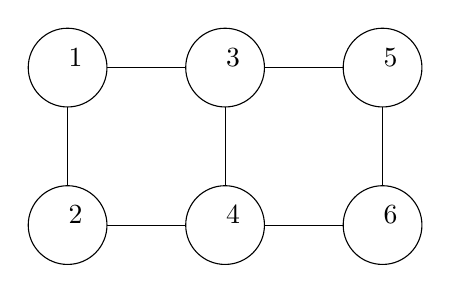
\begin{tikzpicture}
  %ノード1  
  \draw(4,2) circle (0.5)
  node[at={(4.1,2.1)}] {
    \begin{tabular}{c}
      1
    \end{tabular}
  };
  %ノード2  
  \draw(4,0) circle (0.5)
  node[at={(4.1,0.1)}] {
    \begin{tabular}{c}
      2
    \end{tabular}
  };
  %ノード3  
  \draw(6,2) circle (0.5)
  node[at={(6.1,2.1)}] {
    \begin{tabular}{c}
      3
    \end{tabular}
  };
  %ノード4  
  \draw(6,0) circle (0.5)
  node[at={(6.1,0.1)}] {
    \begin{tabular}{c}
      4
    \end{tabular}
  };
  %ノード5  
  \draw(8,2) circle (0.5)
  node[at={(8.1,2.1)}] {
    \begin{tabular}{c}
      5
    \end{tabular}
  };
  %ノード6  
  \draw(8,0) circle (0.5)
  node[at={(8.1,0.1)}] {
    \begin{tabular}{c}
      6
    \end{tabular}
  };
\draw(4,0.5) --(4,1.5);
\draw(6,0.5) --(6,1.5);
\draw(8,0.5) --(8,1.5);
\draw(4.5,0) --(5.5,0);
\draw(4.5,2) --(5.5,2);
\draw(6.5,0) --(7.5,0);
\draw(6.5,2) --(7.5,2);
\end{tikzpicture}

\caption{入力となる重み付き無向グラフの例}
\label{graphexample}
\end{center}
\end{figure}
%%%%%%%%%%%%%%%%%%%%%%%%%%%%%%

%%%%%%%%%%%%%%%%%%%%%%%%%%%%%%
\lstinputlisting[float=t,caption={%
図~\ref{graphexample}のASPファクト表現},%
captionpos=b,frame=single,label=code:graph_example.lp,%
numbers=none,%
breaklines=true,%
columns=fullflexible,keepspaces=true,%
basicstyle=\ttfamily\scriptsize]{code/graph_example.lp}
%%%%%%%%%%%%%%%%%%%%%%%%%%%%%%


本節では,最短ハミルトン閉路問題の例にとって,
入力となる重み付き無向グラフ(図~\ref{graphexample})の
ASP ファクト形式について説明する.
%
このグラフは,頂点数が6,辺の数が7であり,辺に付けられた値は距離を表す.
コード~\ref{code:graph_example.lp}に,ASPファクト形式を示す.
%
アトム\code{node/1}は頂点,\code{edge/2}は辺,\code{cost/3}は距離を表す.
例えば,\code{cost(1,2,3)}は,辺\code{edge(1,2)}の距離が3であることを
表している.

%%%%%%%%%%%%%%%%%%%%%%%%%%%%%%%%%%%%%%%%%%%%%%%%%%%%%%%%%%%%%%%%%%%%%%%
\section{ハミルトン閉路問題の ASP 符号化}\label{hamiltonianasp}
%%%%%%%%%%%%%%%%%%%%%%%%%%%%%%%%%%%%%%%%%%%%%%%%%%%%%%%%%%%%%%%%%%%%%%%

ハミルトン閉路問題は,与えられたグラフの全頂点をちょうど一度ずつ通る閉
路(ハミルトン閉路)が存在するかどうかを判定する問題である.
$G=(V,E)$にハミルトン閉路が存在する必要十分条件は,
以下の2つの制約を満たす部分グラフ$G'=(V,E')$が存在することである.

\begin{itemize}
\item $G'$の各頂点の次数が2 (次数制約)
\item $G'$が連結である (連結制約)
\end{itemize}

本論文では,前者を\textbf{次数制約},後者を\textbf{連結制約}と呼ぶ.
ハミルトン路問題は,ハミルトン閉路問題から始点と終点が一致するという閉
路の条件を取り除いたものである.
ハミルトン路問題では,次数制約は以下のように変わる.

\begin{itemize}
\item 始点と終点の次数が1,他の頂点の次数が2
\end{itemize}

以下では,ハミルトン閉路問題に対する3つの ASP 符号化
\textsf{undirected},\textsf{directed},\textsf{acyclicity}
を提案する.

%%%%%%%%%%%%%%%%%%%%%%%%%%%%%%%%%%%%%%%%%%%%%%%%%%%%%%%%%%%%%%%%%%%%%%%
\subsection{\textsf{undirected}符号化}
%%%%%%%%%%%%%%%%%%%%%%%%%%%%%%%%%%%%%%%%%%%%%%%%%%%%%%%%%%%%%%%%%%%%%%%

%%%%%%%%%%%%%%%%%%%%%%%%%%%%%%
\lstinputlisting[float=t,caption={%
\textsf{undirected}符号化},%
captionpos=b,frame=single,label=code:hamilton1.lp,%
numbers=left,%
breaklines=true,%
columns=fullflexible,keepspaces=true,%
basicstyle=\ttfamily\footnotesize]{code/hamilton1.lp}
%%%%%%%%%%%%%%%%%%%%%%%%%%%%%%

\textsf{undirected}符号化は,ハミルトン閉路問題の次数制約と連結制約を,
ASP の一貫性制約で表した基本的な符号化である.
コード~\ref{code:hamilton1.lp}に,\textsf{undirected}符号化を示す.
この符号化は,ハミルトン閉路問題とハミルトン路問題の両方に対応している.
符号化中の\code{s}は始点の頂点番号,\code{t}は終点の頂点番号を表し,こ
れらは実行時に与えられる.
ここでは,ハミルトン閉路問題(\code{s}=\code{t})の場合について説明する.

\begin{itemize}
\item 1行目のルールは,各辺\code{edge(X,Y)}に対して,その辺がハミルト
  ン閉路に含まれるかどうかを意味するアトム\code{in(X,Y)}を選択子を用い
  て導入している.
\item 次数制約は3行目のルールで表される.このルールは,
  各頂点\code{node(X)}に対して,その次数の和が2に等しいことを個数制約
  を使って表している.
\item 連結制約は11行目のルールで表される.
ある頂点\code{X}が始点\code{s}から到達可能であることを意味する補助アト
ム\code{reached(X)}を導入する.
8行目のルールは,始点\code{s}が到達可能あることを表している.
9行目のルールは,各辺\code{X}--\code{Y}に対して,その辺がハミルトン閉
路に含まれ(\code{in(X,Y)}),かつ,頂点\code{X}が始点から到
達可能であれば(\code{reached(X)}),\code{Y}も到達可能であることを表している.
10行目は9行目と同様であるが,辺\code{Y}--\code{X}の場合を表している.
11行目のルールは,各頂点\code{node(X)}が始点から到達可能でなければな
らないことを一貫性制約を使って表している.
\end{itemize}

%%%%%%%%%%%%%%%%%%%%%%%%%%%%%%%%%%%%%%%%%%%%%%%%%%%%%%%%%%%%%%%%%%%%%%%
\subsection{\textsf{directed}符号化}
%%%%%%%%%%%%%%%%%%%%%%%%%%%%%%%%%%%%%%%%%%%%%%%%%%%%%%%%%%%%%%%%%%%%%%%

%%%%%%%%%%%%%%%%%%%%%%%%%%%%%%
\lstinputlisting[float=t,caption={%
\textsf{directed}符号化},%
captionpos=b,frame=single,label=code:hamilton2.lp,%
numbers=left,%
breaklines=true,%
columns=fullflexible,keepspaces=true,%
basicstyle=\ttfamily\footnotesize]{code/hamilton2.lp}
%%%%%%%%%%%%%%%%%%%%%%%%%%%%%%

\textsf{directed}符号化は,\textsf{undirected}符号化をベースに,
与えられた無向グラフの各辺$u-v$に対して,2つの弧$u\rightarrow v$と
$v\rightarrow u$を対応させることで有向グラフ化して解く符号化である.
コード~\ref{code:hamilton2.lp}に,\textsf{directed}符号化を示す.
前節と同様に,ハミルトン閉路問題(\code{s}=\code{t})の場合について説明する.

\begin{itemize}
\item 1行目では,無向グラフの有向グラフ化を行う.
  与えられた無向グラフの各辺\code{edge(X,Y)}に対して,
  2つの弧\code{edge(X,Y)},\code{edge(Y,X)}を導入した.
\item 2行目のルールは,各弧\code{edge(X,Y)}に対して,その弧がハミルト
  ン閉路に含まれるかどうかを意味するアトム\code{in(X,Y)}を選択子を用い
  て導入している.
\item 次数制約は4,5行目のルールで表される.
  4行目では,各頂点\code{node(X)}に対して,
  その出次数が1に等しいことを個数制約を使って表している.
  5行目では,入次数について4行目と同様の制約を表す.
\item 連結制約は15行目のルールで表される.
  ある頂点\code{X}が始点\code{s}から到達可能であることを意味する
  補助アトム\code{reached(X)}を導入する.
  13行目のルールは,始点\code{s}が到達可能あることを表している.
  14行目のルールは,各弧\code{X}--\code{Y}に対して,その弧がハミルトン閉路
  に含まれ(\code{in(X,Y)}),かつ,頂点\code{X}が始点から
  到達可能であれば(\code{reached(X)}),\code{Y}も到達可能であることを表している.
  15行目のルールは,各頂点\code{node(X)}が始点から到達可能でなければ
  ならないことを一貫性制約を使って表している.
\item 18行目のルールは,解についての対称性を除去する.
  与えられた無向グラフ上の各ハミルトン閉路に対して,
  それを変換した有向グラフ上のハミルトン閉路は対称な2つが存在する.
  これによる解の重複を防ぐために,18行目のルールは,各弧\code{s}--\code{X},
  \code{Y}--\code{s}がハミルトン閉路に含まれるならば(\code{in(s,X),in(Y,s)}),
  \code{X < Y}でなければならないことを,一貫性制約を用いて表している
\end{itemize}

%%%%%%%%%%%%%%%%%%%%%%%%%%%%%%%%%%%%%%%%%%%%%%%%%%%%%%%%%%%%%%%%%%%%%%%
\subsection{\textsf{acyclicity}符号化}
%%%%%%%%%%%%%%%%%%%%%%%%%%%%%%%%%%%%%%%%%%%%%%%%%%%%%%%%%%%%%%%%%%%%%%%

%%%%%%%%%%%%%%%%%%%%%%%%%%%%%%
\lstinputlisting[float=t,caption={%
\textsf{acyclicity}符号化},%
captionpos=b,frame=single,label=code:hamilton3.lp,%
numbers=left,%
breaklines=true,%
columns=fullflexible,keepspaces=true,%
basicstyle=\ttfamily\footnotesize]{code/hamilton3.lp}
%%%%%%%%%%%%%%%%%%%%%%%%%%%%%%

\textsf{acyclicity}符号化は,\textsf{directed}符号化をベースに,
連結の制約に代わる部分閉路禁止制約を組込み非閉路制約で表現した符号化である.
コード~\ref{code:hamilton3.lp}に,\textsf{acyclicity}符号化を示す.
前節と同様に,ハミルトン閉路問題(\code{s}=\code{t})の場合について説明する.

\begin{itemize}
\item 1行目では,無向グラフの有向グラフ化を行う.
  与えられた無向グラフの各辺\code{edge(X,Y)}に対して,
  2つの弧\code{edge(X,Y)},\code{edge(Y,X)}を導入した.
\item 2行目のルールは,各弧\code{edge(X,Y)}に対して,その弧がハミルト
  ン閉路に含まれるかどうかを意味するアトム\code{in(X,Y)}を選択子を用い
  て導入している.
\item 次数制約は4,5行目のルールで表される.
  4行目では,各頂点\code{node(X)}に対して,
  その出次数が1に等しいことを個数制約を使って表している.
  5行目では,入次数について4行目と同様の制約を表す.
\item 部分閉路禁止制約は14行目のルールで表される.
  このルールは,始点でない各頂点\code{X},\code{Y}について,
  弧\code{X}--\code{Y}がハミルトン閉路に含まれるならば(\code{in(X,Y)}),
  そのような弧の集合をもつグラフが閉路をもたないことを,\code{#edge}宣言を用いて表す.
  ようするに,始点(終点)を含まないような閉路を禁止している.
\item 17行目のルールは,解についての対称性を除去する.
  与えられた無向グラフ上の各ハミルトン閉路に対して,
  それを変換した有向グラフ上のハミルトン閉路は対称な2つが存在する.
  これによる解の重複を防ぐために,17行目のルールは,各弧\code{s}--\code{X},
  \code{Y}--\code{s}がハミルトン閉路に含まれるならば(\code{in(s,X),in(Y,s)}),
  \code{X < Y}でなければならないことを,一貫性制約を用いて表している
\end{itemize}

%%%%%%%%%%%%%%%%%%%%%%%%%%%%%%%%%%%%%%%%%%%%%%%%%%%%%%%%%%%%%%%%%%%%%%% 
\section{最短ハミルトン閉路問題のASP符号化}\label{minexpl}
%%%%%%%%%%%%%%%%%%%%%%%%%%%%%%%%%%%%%%%%%%%%%%%%%%%%%%%%%%%%%%%%%%%%%%% 

%% %%%%%%%%%%%%%%%%%%%%%%%%%%%%%%
%% \lstinputlisting[caption =  最適化,label = minimize]{code/obj_minimize.lp}
%% %%%%%%%%%%%%%%%%%%%%%%%%%%%%%%

%%%%%%%%%%%%%%%%%%%%%%%%%%%%%%
\lstinputlisting[float=t,caption={%
最小化},%
captionpos=b,frame=single,label=code:obj_minimize.lp,%
numbers=left,%
breaklines=true,%
columns=fullflexible,keepspaces=true,%
basicstyle=\ttfamily\footnotesize]{code/obj_minimize.lp}
%%%%%%%%%%%%%%%%%%%%%%%%%%%%%%

最短ハミルトン閉路問題の目的関数は,
ハミルトン閉路を構成する各辺の距離の総和である.
コード\ref{code:obj_minimize.lp}は,
その目的関数の最小化を表す.
このコードは,各辺\code{edge(X,Y)}に対して,その辺がハミルトン閉路に
含まれ(\code{in(X,Y)}),その距離が\code{C}である時に(\code{cost(X,Y,C)}),
\code{C}の総和の最小化を,最小化関数を用いて表している.
.
%%%%%%%%%%%%%%%%%%%%%%%%%%%%%%
\lstinputlisting[float=t,caption={%
重み付き無向グラフの有向グラフ化},%
captionpos=b,frame=single,label=code:cost_both.lp,%
numbers=left,%
breaklines=true,%
columns=fullflexible,keepspaces=true,%
basicstyle=\ttfamily\footnotesize]{code/cost_both.lp}
%%%%%%%%%%%%%%%%%%%%%%%%%%%%%%

符号化directed,acyclicityについては,
与えられた無向グラフの各辺\code{edge(X,Y)}に対して,
2つの弧\code{edge(X,Y)},\code{edge(Y,X)}を導入した.
各辺の距離もこれに対応させるために,コード\ref{code:cost_both.lp}
を追加した.
このルールは,各辺\code{X}--\code{Y}の距離を表す\code{cost(X,Y,C)}について,
\code{cost(Y,X,C)}を導入する.
これにより,与えられた無向グラフの各辺\code{edge(X,Y)}の重み\code{C}が
2つの弧\code{edge(X,Y)},\code{edge(Y,X)}にも付与された.

%%%%%%%%%%%%%%%%%%%%%%%%%%%%%%%%%%%%%%%%%%%%%%%%%%%%%%%%%%%%%%%%%%%%%%% 
\section{コスト制約付きハミルトン閉路のASP符号化}
%%%%%%%%%%%%%%%%%%%%%%%%%%%%%%%%%%%%%%%%%%%%%%%%%%%%%%%%%%%%%%%%%%%%%%% 

%%%%%%%%%%%%%%%%%%%%%%%%%%%%%%
\lstinputlisting[float=t,caption={%
コスト制約},%
captionpos=b,frame=single,label=code:cost_constraint.lp,%
numbers=left,%
breaklines=true,%
columns=fullflexible,keepspaces=true,%
basicstyle=\ttfamily\footnotesize]{code/cost_constraint.lp}
%%%%%%%%%%%%%%%%%%%%%%%%%%%%%%

コスト制約付きハミルトン閉路問題は
ハミルトン閉路問題に,距離の総和が所与の閾値以下 (または以上) であること
を制約条件として付加した問題である.
コード\ref{code:const_constraing.lp}のルールは,その制約を表す.
ルール中の\code{c}は閾値を表し,これは実行時に与えられる.
このルールは,各辺\code{edge(X,Y)}に対して,その辺がハミルトン閉路に
含まれ(\code{in(X,Y)}),その距離が\code{C}である時に(\code{cost(X,Y,C)}),
\code{C}の総和が\code{c}以下でなければならないことを,
一貫性制約と重み付き個数制約を用いて表す.

また,\ref{minexpl}と同様に,
符号化directed,acyclicityについては,
アトム\code{cost}についても有向グラフ化に
対応させるためにコード\ref{code:cost_both.lp}を追加した.
%%%%%%%%%%%%%%%%%%%%%%%%%%%%%%%%%%%%%%%%%%%%%%%%%%%%%%%%%%%%%%%%%%%%%%%

%%% Local Variables:
%%% mode: latex
%%% TeX-master: "paper"
%%% End:

  \end{table}
\end{frame}

%%%%%%%%%%%%%%%%%%%%%%%%%%%%%%%%%%%%%%%%%%%%%%%%%%
%% 実験概要--根付き全域森
%%%%%%%%%%%%%%%%%%%%%%%%%%%%%%%%%%%%%%%%%%%%%%%%%%
\begin{frame}{(卒業研究) 実験概要}
  \renewcommand{\thefootnote}{\fnsymbol{footnote}}
  \setcounter{footnote}{1}
  提案手法の有効性を評価するために,以下の実験を行った.
  \begin{itemize}
  \item \structure{\bf 比較するASP符号化:}
    \begin{itemize}
    \item 基本符号化
    \item 改良符号化
    \end{itemize}
  \item \structure{\bf ベンチマーク問題:} 全85問
    \begin{itemize}
    \item DNET\footnote{https://github.com/takemaru/dnet}%
      で公開されている配電網問題 3問 \\ (トポロジ制約のみ,スイッチ数:
      16個,36個,\alert{\bf 468個})
    \item \textit{Graph Coloring and its Generalizations}
      \footnote{https://mat.tepper.cmu.edu/COLOR04/}で公開されている \\
      グラフ彩色問題をベースに,独自に生成した 82問 
      \footnote{各問題に対し,全ノードのうち1/5個をランダムに根として与えた.}\\
      \alert{\bf (20 $\leq$ 辺数 $\leq$ 49,629)}
    \end{itemize}
  \item \structure{\bf ASPシステム:} \textit{clingo-5.4.0} $+$ \textit{trendy}
  \item \structure{\bf 制限時間:} 3600秒/問
  \item \structure{\bf 実験環境:} Mac mini,3.2GHz Intel Core i7,64GBメモリ
  \end{itemize}
\end{frame}
%%%%%%%%%%%%%%%%%%%%%%%%%%%%%%%%%%%%%%%%%%%%%%%%%%
%% カクタスプロット
%%%%%%%%%%%%%%%%%%%%%%%%%%%%%%%%%%%%%%%%%%%%%%%%%%
\begin{frame}{実験結果(1/2) : カクタスプロット}
 \begin{figure}[h]
  \centering
  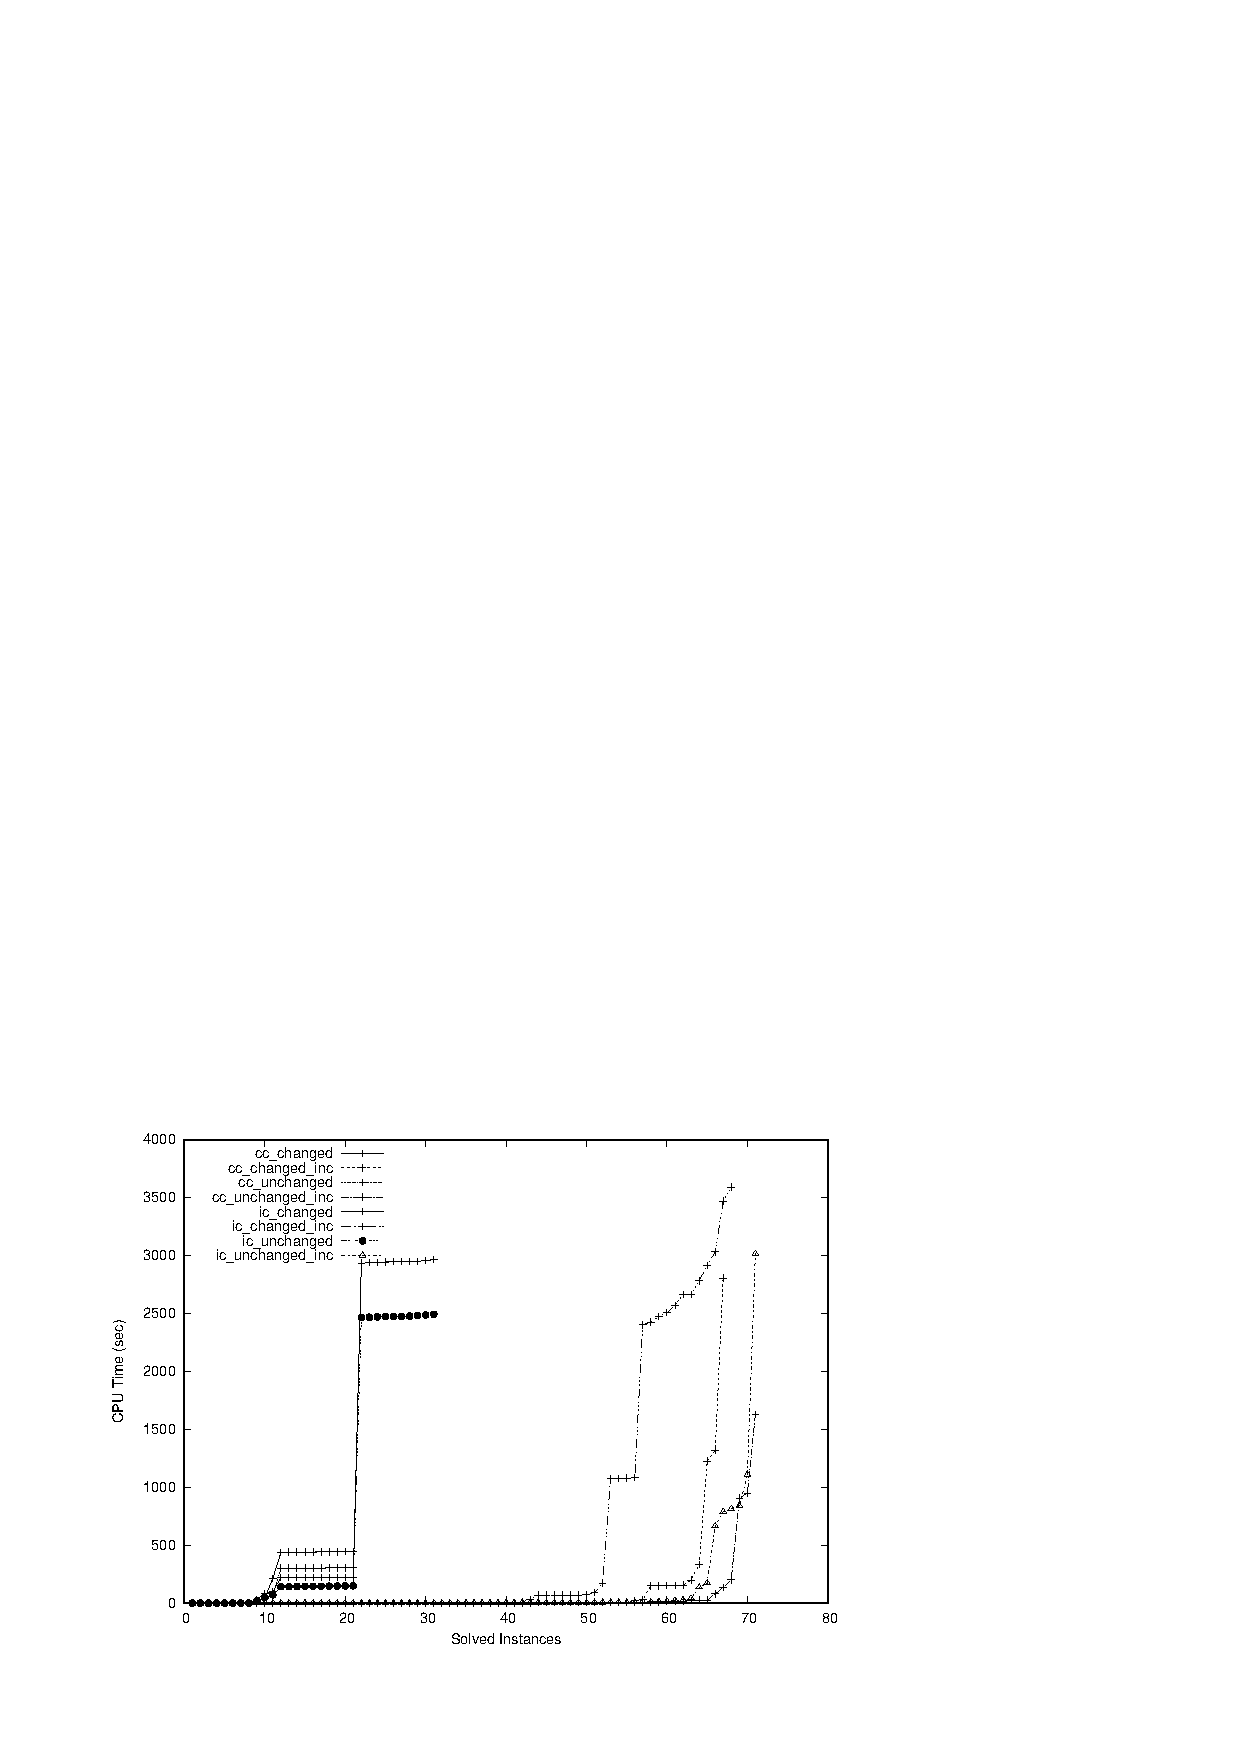
\includegraphics[scale=0.38]{fig/cactus.png}
 \end{figure}\vfill

\begin{itemize}
 \item 改良符号化は,基本符号化と比較して,より多くの問題を高速に解いている.
\end{itemize}
\end{frame}

%%%%%%%%%%%%%%%%%%%%%%%%%%%%%%%%%%%%%%%%%%%%%%%%%%
%% 辺の数の表
%%%%%%%%%%%%%%%%%%%%%%%%%%%%%%%%%%%%%%%%%%%%%%%%%%
\begin{frame}{実験結果(2/2) : 解けた問題数による比較}

\begin{table}[t]
 \centering
 \begin{tabular}[t]{ccccc}
 \rowcolor[RGB]{0,96,0}
 \color{white} 辺の範囲 & \color{white}問題数 & 
		 \color{white}基本符号化 & \color{white}改良符号化 & \color{white}有向符号化\\
 %%%%%%%%
 \rowcolor[RGB]{230,239,230}
 ~~~~\;\:1 ~ 1,000 & 30 & \alert{30} & \alert{30} & \alert{30} \\
 \rowcolor[RGB]{196,230,196}
 1,001 ~ 4,000 & 20 & \alert{20} & \alert{20} & \alert{20} \\
 \rowcolor[RGB]{230,239,230}
 4,001 ~ 7,000 & 11 & 9 & 10 & \alert{11} \\
 \rowcolor[RGB]{196,230,196}
 ~\:7,001 ~ 10,000 & 8 & 4 & 6 &\alert{7} \\
 \rowcolor[RGB]{230,239,230}
 10,001 ~ 20,000 & 9 & 2 & 5 &\alert{9} \\
 \rowcolor[RGB]{196,230,196}
 20,001 ~ 30,000 & 2 & 1 & \alert{2} & \alert{2} \\
 \rowcolor[RGB]{230,239,230}
 30,001 ~ 40,000 & 1 & 0 & 0 & \alert{1} \\
 \rowcolor[RGB]{196,230,196}
 40,001 ~ 50,000 & 4 & 0 & 2 & \alert{4} \\
 %%%%%%%% 合計
 \noalign{\hrule height 0.5pt}
 \rowcolor[RGB]{230,239,230}
 計 & 85 & 66 & 75 & \alert{84} \\
 
\end{tabular}

\end{table}\vfill

\begin{itemize}
\item 辺の数が4,000を超える問題では,改良符号化がより多くの問題を解いている.
\item 改良符号化は,辺の数が40,000を超える問題も解けている.
\item 大規模な問題に対する改良符号化の優位性が確認できた.
\end{itemize}
\end{frame}

%%%%%%%%%%%%%%%%%%%%%%%%%%%%%%%%%%%%%%%%%%%%%%%%%%
%% 遷移問題
%%%%%%%%%%%%%%%%%%%%%%%%%%%%%%%%%%%%%%%%%%%%%%%%%%
\begin{frame}{根付き全域森遷移問題の例}
  \begin{itemize}
  \item \structure{\bf 遷移制約}: 各ステップ$t$で変更可能な辺の数を
    $d=2$個以下とする.
  \end{itemize}
\begin{exampleblock}{}
 \begin{figure}[h]
  %\renewcommand{\arraystretch}{0.9}
  \tabcolsep = 3mm  
  \centering
  \begin{tabular}{ccc}
   \onslide<1-> $t=0$ (スタート状態) & & \onslide<2> $t=1$\\
   \onslide<1-> \scalebox{0.8}{\input{tikz/tikz-trans-1}}
   & \onslide<2> \lw{$\Rightarrow$} & 
	\onslide<2> \scalebox{0.8}{\input{tikz/tikz-trans-2}}\\
   & & \onslide<2> \lower1ex\hbox{$\Downarrow$} \\
   & & \\
   \onslide<1-> \scalebox{0.8}{%%%%%%%%%%%%%%%%%%%%%%%%%%%%%%%%%%%%%%%%%%%%%%%%%%
% 実行例(t=3) (第6章で使う)
%%%%%%%%%%%%%%%%%%%%%%%%%%%%%%%%%%%%%%%%%%%%%%%%%%
\begin{tikzpicture}[scale=0.6]

 % 設定
 \tikzset{node/.style={circle,draw=black,fill=white}}

 \definecolor{edge1}{RGB}{191,0,0}
 \definecolor{node1}{RGB}{249,200,200}
 \definecolor{edge3}{RGB}{38,38,134}
 \definecolor{node3}{RGB}{200,200,249}

 % 補助線
 % \draw [help lines,blue] (0,0) grid (20,6);

 % node %
 \node[circle, ultra thick, draw=edge1, fill=node1](out1){1};
 \node[node, fill=node3, right=of out1] (out2){2};
 \node[circle, ultra thick, draw=edge3,fill=node3, right=of out2](out3){3};
 \node[node, fill=node3, below=of out1] (out4){4};
 \node[node, fill=node3, below=of out2] (out5){5};
 \node[node, fill=node3, below=of out3] (out6){6};

 \foreach \u / \v in {}
 \draw [very thick, edge1] (\u) -- (\v);

 \foreach \u / \v in {out2/out3,out2/out5,out4/out5,out5/out6}
 \draw [very thick, edge3](\u) -- (\v);
\end{tikzpicture}

%%%%%%%%%%%%%%%%%%%%%%%%%%%%%%%%%%%%%%%%%%%%%%%%%%%%%%%%%%
%%% Local Variables:
%%% mode: japanese-latex
%%% TeX-master: paper.tex
%%% End:
}
   & \onslide<2> \lw{$\Leftarrow$} &
   \onslide<2> \scalebox{0.8}{\input{tikz/tikz-trans-3}}\\
   \onslide<1->$t= \only<1>{\ ?} \only<2>{\structure{\bf 3}} $ (ゴール状態) 
   & & \onslide<2> $t=2$
  \end{tabular}
 \end{figure}
\end{exampleblock}
\end{frame}

\backupend

%%% Local Variables:
%%% mode: japanese-latex
%%% TeX-master: "slide.tex"
%%% End:
